\documentclass[11pt,a4paper]{article}

\usepackage[utf8]{inputenc}
\usepackage[T1]{fontenc}
\usepackage{amsmath,amssymb,amsthm}
\usepackage{geometry}
\usepackage{tikz}
\usetikzlibrary{calc}
\usepackage{hyperref}
\usepackage{enumitem}
\usepackage{booktabs}
\usepackage{longtable}
\usepackage{algorithm}
\usepackage{algpseudocode}

\geometry{margin=2.6cm}
\emergencystretch=3em
\renewcommand{\_}{\textunderscore\discretionary{}{}{}}
\hypersetup{colorlinks=true, linkcolor=blue!50!black, citecolor=blue!50!black, urlcolor=blue!50!black}

\newtheorem{proposition}{Proposition}
\newtheorem{definition}{Definition}

\newcommand{\R}{\mathbb{R}}
\newcommand{\dif}{\mathrm{d}}
\newcommand{\grad}{\nabla}

\title{Mathematical Foundations and Implementation of\\
Area Minimization under a Volume Constraint\\[0.3em]
\large Droplet relaxation with wetting, a moving obstacle and\\
heterogeneous substrates -- Theory (Part~I) and Implementation (Part~II)}
\author{Companion document to the \emph{Droplet Relaxer} project}
\date{\today}

\begin{document}
\maketitle

\begin{abstract}
\noindent
This document describes the \texttt{droplet\_relaxer} program: the
relaxation of a liquid droplet on a flat substrate -- optionally pulled
by a moving rigid sphere -- to its minimal-energy shape at fixed volume,
implemented as discrete gradient descent on a triangle mesh, at its core
the same principle as Ken Brakke's \emph{Surface Evolver}.
\textbf{Part~I (Theory)} is independent of the code: the continuous
variational problem, the interfacial (wetting) energies including a
circular wettability anomaly, the force on the sphere, the discretization
with explicit derivations of all gradients, and the optimization theory
(constraints, Sobolev gradients, step control).
\textbf{Part~II (Implementation)} describes how this is realized in the
program: module structure, meshes and scaling, assembly of energies and
forces in each iteration, the solver, remeshing, visualization and
output, the purely numerical ingredients that have no physical origin,
validation results and known limitations. \textbf{Part~III} compares the
project with the Surface Evolver and lists possible extensions.
\end{abstract}

\tableofcontents

% ======================================================================
\section{Motivation and Overview}
% ======================================================================

A liquid droplet on a substrate takes on the shape that
minimizes its interfacial energy while its volume stays constant (liquid
is incompressible). Since the liquid/vapor energy is proportional to area, this
leads to a classical \emph{constrained variational problem}:
\begin{equation}
  \min_{\Sigma} \; A[\Sigma] \quad \text{subject to} \quad V[\Sigma] = V_0,
  \label{eq:problem}
\end{equation}
where $\Sigma$ is a surface with a boundary curve (the contact line) on
the substrate, $A[\Sigma]$ is its area, and $V[\Sigma]$ is the enclosed
volume. Wetting adds energies on the contact area with the substrate and
with a rigid obstacle (Section~\ref{sec:interfaces}).

Kenneth Brakke's Surface Evolver \cite{Brakke1992} solves exactly this
problem (and substantially more general variants of it) numerically,
by discretizing the surface as a triangle mesh and iteratively moving
the vertices along the negative gradient of the energy -- a discrete
gradient descent. Our program mirrors the same principle, with two
improvements over the simplest approach: a Sobolev preconditioning of
the gradient (Section~\ref{sec:sobolev}) and a penalty formulation of
the volume constraint (Section~\ref{sec:constraint}).

\paragraph{How this document is organized.}
\emph{Part~I} states the model and derives the mathematics; it
contains no program names or parameter values and would be valid for any
implementation. \emph{Part~II} states what the program does with it:
which quantities are computed where, which numerical devices were added
that are \emph{not} implied by the theory, how the output is produced and
how it was checked. Cross-references between the parts point from
each implementation item to the equation it realizes
(Table~\ref{tab:mapping} collects them).

\part{Theory}

% ======================================================================
\section{The Continuous Variational Problem}
\label{sec:continuous-problem}
% ======================================================================


\subsection{The Area Functional and Its First Variation}

Let $\Sigma \subset \R^3$ be a smooth, oriented surface with unit
normal $n$. Consider a family of surfaces $\Sigma_t$ obtained by
displacing every point along the normal:
\begin{equation}
  x(t) = x_0 + t\,\varphi(x_0)\, n(x_0), \qquad x_0 \in \Sigma,
\end{equation}
with a scalar "speed function" $\varphi$. The first variation of the
area functional $A[\Sigma_t] = \int_{\Sigma_t} \dif A$ under this
perturbation is a classical result of differential geometry:
\begin{equation}
  \left.\frac{\dif}{\dif t}\right|_{t=0} A[\Sigma_t]
  = -\int_{\Sigma} H \,\varphi \; \dif A,
  \label{eq:first-variation-area}
\end{equation}
where $H = \kappa_1 + \kappa_2$ is the mean curvature (here defined as
the sum of the principal curvatures). Equation
\eqref{eq:first-variation-area} states that the $L^2$-gradient of the
area functional with respect to normal displacements is
\begin{equation}
  \grad A \;=\; -H\, n.
  \label{eq:area-gradient-continuous}
\end{equation}
The steepest descent $\partial x/\partial t = -\grad A = H n$ is thus
exactly the \emph{mean curvature flow} -- precisely the process that
Brakke described mathematically, rigorously, within the framework of
geometric measure theory, in his dissertation \cite{Brakke1978} (from
which the Surface Evolver later grew).

\subsection{The Volume Constraint}

Displacing the surface by $\varphi\,n$ changes the enclosed volume, to
first order, by
\begin{equation}
  \left.\frac{\dif}{\dif t}\right|_{t=0} V[\Sigma_t]
  = \int_{\Sigma} \varphi \; \dif A,
  \qquad\text{i.e.}\qquad
  \grad V = n.
  \label{eq:volume-gradient-continuous}
\end{equation}
For the minimization problem \eqref{eq:problem}, the Lagrange
multiplier method gives: at a critical point there exists
$\lambda \in \R$ such that
\begin{equation}
  \grad A - \lambda \,\grad V = 0
  \quad\Longleftrightarrow\quad
  H = \lambda = \text{const.}
  \label{eq:cmc}
\end{equation}
This is the classical theorem that area-minimizing surfaces under a
fixed volume constraint have \emph{constant mean curvature} (spherical
caps, soap bubbles) -- the Lagrange multiplier $\lambda$ is physically
the internal pressure (the Young--Laplace law).

\subsection{Boundary Condition at the Contact Line}
\label{sec:contact-line}

At the boundary $\partial\Sigma$ (the contact line), there are two
standard cases:
\begin{itemize}
  \item \textbf{Pinned boundary (Dirichlet):} $\partial\Sigma$ is fixed
    in advance, e.g.\ a circle on the substrate.
  \item \textbf{Free contact angle (Neumann-type):} $\partial\Sigma$ is
    allowed to move freely on the substrate, but there is a substrate
    energy $(\gamma_{sl}-\gamma_{sv})\cdot(\text{wetted area})$. The
    first variation then leads to Young's equation
    $\cos\theta = (\gamma_{sv}-\gamma_{sl})/\gamma_{lv}$ for the
    equilibrium contact angle $\theta$.
\end{itemize}
In the model treated here the boundary condition is a mixture of the
two: the contact line is Dirichlet-constrained only in the direction
\emph{normal to the substrate} (it must stay on the wall, $z=0$) but is
otherwise free to slide within the substrate plane, with the
free-contact-angle substrate energy added explicitly (Section~\ref{sec:wall-energy}).
Without that energy term the boundary reduces to a pure natural
(Neumann) condition and settles at $\theta=90^\circ$; the contact line is never
pinned (fixed radius) in this model. The discrete degree-of-freedom
restriction is described in Section~\ref{sec:boundary-discrete}.

% ======================================================================
\section{Interfacial Energies and Wetting}
\label{sec:interfaces}
% ======================================================================

This section states the physical energies that go beyond the pure area
functional: the wall (liquid/solid) energy, a substrate whose wettability
varies in space, the energy of the liquid in contact with a rigid sphere,
and the force the liquid exerts on that sphere. All of it is
formulated for smooth surfaces; the discrete counterparts follow in
Section~\ref{sec:discrete-contact}.

\subsection{Young's Energy and the Wall Energy}
\label{sec:wall-energy}

Let the liquid be bounded by a liquid/vapor surface $\Sigma_{lv}$
(area $A_{lv}$) and a wetted region of the substrate (liquid/solid
interface, area $A_{sl}$). With the three interfacial tensions
$\gamma_{lv},\gamma_{sl},\gamma_{sv}$ and a substrate of total area
$A_{\mathrm{wall}}$ (a constant),
\begin{equation}
  E = \gamma_{lv}A_{lv} + \gamma_{sl}A_{sl} + \gamma_{sv}(A_{\mathrm{wall}}-A_{sl})
  = \gamma_{lv}A_{lv} - (\gamma_{sv}-\gamma_{sl})A_{sl} + \mathrm{const}.
\end{equation}
Moving the contact line outward by $\delta$ per unit length changes
$A_{sl}$ by $+\delta$ and, for a liquid/vapor surface meeting the wall at
the interior angle $\theta$, $A_{lv}$ by $\cos\theta\,\delta$, so
stationarity gives \emph{Young's equation}
\begin{equation}
  \gamma_{sv}-\gamma_{sl} = \gamma_{lv}\cos\theta_Y .
  \label{eq:young}
\end{equation}
Writing $\kappa:=\cos\theta_Y$, the total interface energy is therefore
\begin{equation}
  E \;=\; \gamma_{lv}A_{lv} \;-\; \kappa\,\gamma_{lv}\,A_{sl}.
  \label{eq:total-energy}
\end{equation}
A positive $\kappa$ (more wetting, $\theta_Y<90^\circ$) \emph{rewards} a
larger wetted area; $\kappa=0$ ($\theta_Y=90^\circ$) means no wall
energy at all. For the pure area problem of
Section~\ref{sec:continuous-problem} we set $\gamma_{lv}=1$: a constant
factor does not change the minimizer. The wall part alone is
\begin{equation}
  E_{\mathrm{wall}} = -\kappa\,\gamma_{lv}\, A_{\mathrm{proj}},
  \label{eq:wall-energy}
\end{equation}
where $A_{\mathrm{proj}}=A_{sl}$ is the area enclosed by the contact line's
projection onto the (flat) substrate plane. By Green's theorem this
area is a closed line integral over the contact line $\partial\Sigma$ --
the planar analogue of the divergence-theorem trick used for the
volume (Section~\ref{sec:discrete-volume}):
\begin{equation}
  A_{\mathrm{proj}} = \frac{1}{2}\oint_{\partial\Sigma} (x\,\dif y - y\,\dif x).
  \label{eq:green}
\end{equation}
Consequently the wall energy needs no substrate surface mesh at all: it
depends only on the contact line.

\subsection{A Substrate with Spatially Varying Wettability}
\label{sec:anomaly-theory}

If the Young angle varies over the substrate, $\kappa=\kappa(x,y)$,
the wall energy generalizes to an integral over the wetted region
$\Omega_{\mathrm{wet}}$ (the region of the plane enclosed by the contact
line):
\begin{equation}
  E_{\mathrm{wall}} = -\gamma_{lv}\int_{\Omega_{\mathrm{wet}}}\kappa(x,y)\,\dif A .
  \label{eq:wall-heterogeneous}
\end{equation}
Consider a homogeneous wall ($\kappa_0=\cos\theta_0$) with a circular
anomaly of centre $\mathbf p$, radius $r$ and angle $\theta_a$
($\kappa_a=\cos\theta_a$). With a smooth indicator $s(\rho)$ of the disc,
$\rho=|\mathbf x-\mathbf p|$, $\kappa=\kappa_0+(\kappa_a-\kappa_0)\,s$, and the
energy splits into the homogeneous part \eqref{eq:wall-energy} and
\begin{equation}
  E_{\mathrm{anom}} = -\gamma_{lv}(\kappa_a-\kappa_0)\int_{\Omega_{\mathrm{wet}}} s(\rho)\,\dif A .
  \label{eq:anomaly-energy}
\end{equation}
The indicator is $s=1$ for $\rho\le r-h$, $s=0$ for $\rho\ge r+h$ and, in the
transition zone of total width $2h$, the quintic ``smootherstep''
\begin{equation}
  s = 1-(10u^3-15u^4+6u^5),\qquad u=\frac{\rho-(r-h)}{2h}\in[0,1],
  \label{eq:smootherstep}
\end{equation}
which is $C^2$ (so $E_{\mathrm{anom}}$ has a continuous second derivative
with respect to the contact line). The width is parametrized as
$2h=f\,r$ with a fraction $f$ of the radius.

\paragraph{Reduction to a contact-line integral.} Since $s$ is radial, the
area integral can again be written as a boundary integral. Let
$S(\rho)=\int_0^\rho s(r')\,r'\,\dif r'$ (a polynomial on the transition zone,
closed form) and define the vector field
\begin{equation}
  \mathbf P(\mathbf x)=\frac{S(\rho)}{\rho^2}\,(\mathbf x-\mathbf p).
  \label{eq:flux-field}
\end{equation}
Its divergence is $\operatorname{div}\mathbf P=\frac1\rho\frac{\dif}{\dif\rho}\big(\rho\cdot S/\rho\big)
=S'(\rho)/\rho=s(\rho)$, hence by the divergence theorem
\begin{equation}
  \int_{\Omega_{\mathrm{wet}}} s\,\dif A=\oint_{\partial\Sigma}\mathbf P\cdot\mathbf n\,\dif l,
  \label{eq:anomaly-flux}
\end{equation}
with $\mathbf n$ the outward normal of the contact line in the plane.
(At $\rho\to0$, $\mathbf P\to(\mathbf x-\mathbf p)/2$, so the field is regular.)
The first variation of this boundary integral under a displacement
$\delta\mathbf x$ of the contact line is
\begin{equation}
  \delta\!\int_{\Omega_{\mathrm{wet}}} s\,\dif A=\oint_{\partial\Sigma} s\,(\mathbf n\cdot\delta\mathbf x)\,\dif l,
  \label{eq:anomaly-variation}
\end{equation}
that is, the local Young force $-\gamma_{lv}\kappa(\mathbf x)\,\mathbf n$ at each
point of the contact line, now with the local wettability $\kappa(\mathbf x)$.

\paragraph{Consequences.} (i) A patch lying completely \emph{inside} the
wetted region has no effect: only the part of the wetted region that the contact
line sweeps over contributes to a change of the energy. (ii) For a hydrophilic
patch ($\theta_a<\theta_0$) the energy as a function of the droplet position has
a well of depth about $\gamma_{lv}(\kappa_a-\kappa_0)A_{\mathrm{covered}}$, for a
hydrophobic one a hill of that height. (iii) The model has no contact-angle
hysteresis: pinning at the patch edge arises only from this energy barrier.

\subsection{Wetting Energy on a Rigid Sphere}
\label{sec:sphere-wetting-theory}

The same Young-type energy applies where the liquid touches a rigid sphere
of radius $R$ and centre $\mathbf c$: the wetted part of the sphere
(liquid/solid interface, area $A_{\mathrm{patch}}$) lowers or raises the energy,
\begin{equation}
  E_{\mathrm{wetting}} = -\kappa_{\mathrm{sphere}}\,\gamma_{lv}\,A_{\mathrm{patch}},
  \qquad \kappa_{\mathrm{sphere}}=\cos\theta_{Y,\mathrm{sphere}},
  \label{eq:sphere-wetting-energy-cont}
\end{equation}
and the liquid/vapor area excludes the wetted facets. Unlike the plane,
a sphere has no simple global vector potential for its area form, so the
trick of Eq.~\eqref{eq:green} does not carry over directly -- an arbitrarily
oriented loop on a sphere is exactly the setting of the holonomy term in the
Gauss--Bonnet theorem. The way out is to use Gauss--Bonnet itself: for a
simple loop $\gamma$ on the unit sphere bounding a region $D$,
$\int_D K\,\dif A = 2\pi-\oint_\gamma\kappa_g\,\dif s$ with $K=1$, i.e.\ the
\emph{solid angle} enclosed by the loop is
\begin{equation}
  \Omega = 2\pi-\oint_\gamma \kappa_g\,\dif s ,
  \qquad A_{\mathrm{patch}}=R^2\,\Omega ,
  \label{eq:gauss-bonnet}
\end{equation}
which refers only to the loop itself (its geodesic curvature), not to any global
potential or preferred direction. The price is that ``the enclosed side'' must be
unambiguous, i.e.\ the loop must be small enough (it must not wrap around the
sphere) and must be a single simple loop.

\subsection{The Force on the Sphere}
\label{sec:force-theory}

For a quasi-static process the force of the liquid on the sphere follows
from virtual work, $\mathbf F=-\partial E/\partial\mathbf c$: the energy
change per displacement of the sphere centre. The configuration of the
liquid depends on $\mathbf c$ as well, but at equilibrium the liquid
minimizes $E$ for each $\mathbf c$, so by the envelope argument only the
\emph{explicit} dependence of $E$ on $\mathbf c$ is needed, namely
(i) the contact/collision terms and the Young term on the sphere patch,
which depend on $\mathbf v-\mathbf c$, and (ii) the reaction of the
constraint that holds the wetted liquid on the sphere surface, which carries
the liquid pressure on the patch and the radial pull of the contact line.
Out of equilibrium the same expression is the instantaneous force the
current liquid configuration exerts on the sphere (force balance).

\paragraph{Symmetry.} On a homogeneous substrate the whole system is invariant
under lateral translations of sphere and droplet together, so the equilibrium
energy $E^*(\mathbf c)$ does not depend on the lateral position and
$F_x=F_y=0$ at equilibrium. A \emph{lateral} force at equilibrium requires
a symmetry-breaking substrate: with a wettability anomaly
(Section~\ref{sec:anomaly-theory}) $E^*(X)$ has a well or hill and
$F_x=-\dif E^*/\dif X$. What a moving sphere in a real liquid experiences as
friction additionally contains viscous dissipation and contact-angle
hysteresis, neither of which is in this energy model.

\subsection{Centre of Mass}

For a closed liquid surface the centroid of the enclosed (homogeneous) liquid is,
by the divergence theorem applied componentwise,
\begin{equation}
  \mathbf r_{\mathrm{COM}}=\frac{1}{V}\int_{\mathrm{liquid}}\mathbf x\,\dif V,
  \label{eq:com}
\end{equation}
which the discrete formula of Section~\ref{sec:discrete-com} evaluates from the
boundary alone. The offset of the centre of mass from the sphere centre in the
substrate plane, $(d_x,d_y)=\mathbf r^{\mathrm{COM}}_{xy}-\mathbf c_{xy}$, $d=\sqrt{d_x^2+d_y^2}$, is
a convenient measure of how far the droplet lags behind or leads the sphere.


% ======================================================================
\section{Discretization: The Surface as a Simplicial Complex}
\label{sec:discretization}
% ======================================================================
\subsection{Notation}

We replace the smooth surface $\Sigma$ with a triangle mesh: a set of
vertices $\{v_i\}_{i=1}^{N} \subset \R^3$ and a set of triangles
(facets) $T$, where each triangle $t \in T$ is given by an ordered
triple $(i,j,k)$ of vertex indices. This piecewise-linear surface is
exactly the \emph{simplicial complex} that the Surface Evolver also
uses as its data structure.

\begin{figure}[h]
\centering
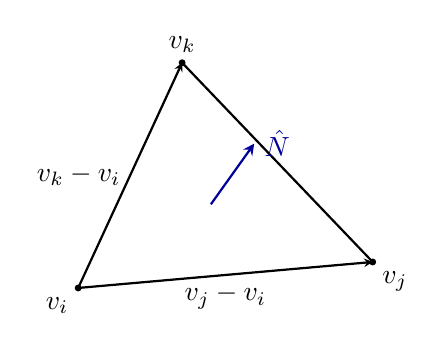
\begin{tikzpicture}[scale=2.2, >=stealth]
  \coordinate (vi) at (0,0);
  \coordinate (vj) at (1.7,0.15);
  \coordinate (vk) at (0.6,1.3);
  \draw[thick] (vi) -- (vj) -- (vk) -- cycle;
  \fill (vi) circle (0.02) node[below left] {$v_i$};
  \fill (vj) circle (0.02) node[below right] {$v_j$};
  \fill (vk) circle (0.02) node[above] {$v_k$};
  \coordinate (centroid) at ($ (vi)!0.333!(vj)!0.333!(vk) $);
  \coordinate (mid) at (0.766,0.483);
  \draw[->, thick, blue!60!black] (mid) -- ++(0.25,0.35) node[right] {$\hat N$};
  \draw[->, dashed] (vi) -- (vj) node[midway, below] {$v_j-v_i$};
  \draw[->, dashed] (vi) -- (vk) node[midway, left] {$v_k-v_i$};
\end{tikzpicture}
\caption{A triangle $t=(i,j,k)$ with edge vectors and unit normal
  $\hat N$. The triangle's area and its gradient with respect to each
  vertex are derived in Section~\ref{sec:area-gradient}.}
\label{fig:triangle}
\end{figure}

\subsection{The Discrete Area Functional}

For a triangle $t=(i,j,k)$ we define the (unnormalized) normal vector
\begin{equation}
  N_t \;=\; (v_j - v_i) \times (v_k - v_i),
  \qquad
  \hat N_t = \frac{N_t}{|N_t|},
\end{equation}
so that its area is $\mathrm{Area}_t = \tfrac{1}{2}|N_t|$. The
discrete area functional is the sum over all triangles:
\begin{equation}
  A(x) \;=\; \sum_{t \in T} \mathrm{Area}_t
  \;=\; \frac{1}{2}\sum_{t=(i,j,k) \in T} \big|(v_j-v_i)\times(v_k-v_i)\big|,
  \label{eq:discrete-area}
\end{equation}
where $x = (v_1,\dots,v_N) \in \R^{3N}$ is the vector of all vertex
coordinates.

\subsection{Derivation of the Area Gradient}
\label{sec:area-gradient}

We compute $\grad_{v_i} \mathrm{Area}_t$ for a fixed triangle
$t=(i,j,k)$. With $a := v_j,\, b:= v_k$ held constant and $x := v_i$
the variable, we have $N_t(x) = (a-x)\times(b-x)$. The directional
derivative in direction $h$ is
\begin{align}
  \dif N_t[h]
  &= (-h)\times(b-x) + (a-x)\times(-h) \notag\\
  &= (b-x)\times h - (a-x)\times h \notag\\
  &= \big[(b-x)-(a-x)\big]\times h
  \;=\; (b-a)\times h.
  \label{eq:dN}
\end{align}
Since $\mathrm{Area}_t = \tfrac12 |N_t|$ and $\dif|N_t|[h] = \hat N_t
\cdot \dif N_t[h]$ (the derivative of a norm is the projection onto
the unit direction), \eqref{eq:dN} gives
\begin{equation}
  \dif \mathrm{Area}_t[h]
  = \tfrac12\, \hat N_t \cdot \big[(b-a)\times h\big]
  = \tfrac12\, h \cdot \big[\hat N_t \times (b-a)\big],
\end{equation}
where we used the cyclic invariance of the scalar triple product
$u\cdot(v\times w) = w\cdot(u\times v)$. Since the directional
derivative is exactly $h \cdot \grad_{v_i}\mathrm{Area}_t$, we can read
off the gradient directly:
\begin{equation}
  \boxed{\;
  \grad_{v_i} \mathrm{Area}_t
  \;=\; \tfrac12\, \hat N_t \times (v_k - v_j)
  \;=\; \tfrac12\,(v_j - v_k)\times \hat N_t
  \;}
  \label{eq:area-grad-vi}
\end{equation}
By cyclically permuting the roles of $i,j,k$ (the triangle is
symmetric under cyclic relabeling), we immediately obtain
\begin{equation}
  \grad_{v_j} \mathrm{Area}_t = \tfrac12(v_k-v_i)\times \hat N_t,
  \qquad
  \grad_{v_k} \mathrm{Area}_t = \tfrac12(v_i-v_j)\times \hat N_t.
  \label{eq:area-grad-vjvk}
\end{equation}
The total gradient of $A(x)$ with respect to a vertex $v_i$ is the sum
of \eqref{eq:area-grad-vi}--\eqref{eq:area-grad-vjvk} over all
triangles containing $v_i$ (the so-called "1-ring" around $v_i$).

\subsection{The Discrete Volume Functional}
\label{sec:discrete-volume}

For a closed surface, the divergence theorem with the vector field
$F(x) = x/3$ (which satisfies $\mathrm{div}\,F \equiv 1$) gives
\begin{equation}
  V = \int_{\mathrm{volume}} 1 \,\dif V
  = \int_{\Sigma} \tfrac13\, x\cdot n \;\dif A.
\end{equation}
On a triangle $t=(i,j,k)$ (with matching orientation), this surface
integral reduces to the well-known tetrahedron volume relative to the
origin:
\begin{equation}
  V_t = \tfrac16\, v_i \cdot (v_j \times v_k),
\end{equation}
and the total volume is the sum
\begin{equation}
  V(x) = \frac16 \sum_{t=(i,j,k)\in T} v_i \cdot (v_j\times v_k).
  \label{eq:discrete-volume}
\end{equation}
For a \emph{closed} surface, this value is independent of the choice
of origin (the contributions of the "missing" opposite side cancel out
telescopically). In our case (an open surface above a substrate plane
$z=0$ passing through the origin), $x\cdot n = 0$ holds for every
point on the substrate -- the "cap" contributes exactly zero to the
sum \eqref{eq:discrete-volume}, which is why we can compute the volume
using only the free (upper) droplet surface, without explicitly
triangulating the substrate cap.

\subsection{Derivation of the Volume Gradient}

Equation \eqref{eq:discrete-volume} is linear in each individual
vertex (with the other two held fixed), so the derivative is
immediate:
\begin{equation}
  \frac{\partial}{\partial v_i}\big[v_i\cdot(v_j\times v_k)\big]
  = v_j \times v_k.
\end{equation}
For the derivatives with respect to $v_j$ and $v_k$, we again use the
cyclic symmetry of the scalar triple product,
$v_i\cdot(v_j\times v_k) = v_j\cdot(v_k\times v_i) = v_k\cdot(v_i\times v_j)$,
and obtain
\begin{equation}
  \boxed{\;
  \grad_{v_i} V_t = \tfrac16\, v_j\times v_k, \qquad
  \grad_{v_j} V_t = \tfrac16\, v_k\times v_i, \qquad
  \grad_{v_k} V_t = \tfrac16\, v_i\times v_j.
  \;}
  \label{eq:volume-grad}
\end{equation}

\subsection{Connection to Discrete Mean Curvature}
\label{sec:mean-curvature}

A well-known result of discrete differential geometry \cite{Meyer2003}
states that the area gradient at a vertex is proportional to the mean
curvature vector:
\begin{equation}
  \grad_{v_i} A \;\approx\; 2\,H(v_i)\, n(v_i)\, A_{\mathrm{mixed}}(v_i),
  \label{eq:curvature-from-gradient}
\end{equation}
where $A_{\mathrm{mixed}}(v_i)$ is a suitable "mixed"
(Voronoi-like) area assigned to the vertex. This is consistent with
\eqref{eq:area-gradient-continuous}: the continuous gradient $-Hn$
reappears discretely as a weighted mean curvature vector. We
pragmatically approximate $A_{\mathrm{mixed}}(v_i)$ as one third of
the sum of the adjacent triangle areas (instead of the exact Voronoi
cell) and obtain from it the \emph{unsigned} curvature
\begin{equation}
  H(v_i) \;\approx\; \frac{|\grad_{v_i} A|}{2\,A_{\mathrm{mixed}}(v_i)},
\end{equation}
which is used to colour the surface in the visualization -- without having to implement a
separate curvature operator.

\paragraph{A boundary caveat.} Relation
\eqref{eq:curvature-from-gradient} assumes a \emph{complete} triangle
fan around $v_i$ and is only exact for interior vertices. At a
boundary vertex (a point on the contact line), the fan is incomplete,
and the raw area gradient there picks up an additional contribution
related to the geodesic curvature of the boundary curve itself --
unrelated to the true surface curvature $H$. Numerically, this
contribution can be an order of magnitude larger than the genuine
curvature signal (in a typical run, boundary vertices show apparent
curvatures around $60$--$70$ versus a true local value near $0.5$),
which saturates the color scale and produces a spuriously bright rim
in the visualization. The program corrects for this by
replacing each boundary vertex's displayed curvature with the average
of its interior neighbors' values; this is a purely
cosmetic fix for the color map and does not affect the optimization
itself, which never uses \eqref{eq:curvature-from-gradient} directly
(it works with the exact area/volume gradients of
Section~\ref{sec:area-gradient}).


\subsection{Discrete Contact-Line Energies}
\label{sec:discrete-contact}

This subsection gives the discrete counterparts of the energies of
Section~\ref{sec:interfaces}. The contact line is the ordered closed polygon
$p_1,\dots,p_n$ of dome vertices on the substrate (for the wall) or on
the sphere (for the wetted patch).

\paragraph{Wall energy: shoelace formula.} The wetted substrate area is the
area of the planar polygon given by the $(x,y)$ coordinates of the contact line,
\begin{equation}
  A_{sl}=A_{\mathrm{proj}}=\frac12\sum_{i}\big(x_i y_{i+1}-x_{i+1}y_i\big),
  \label{eq:shoelace}
\end{equation}
($i$ cyclic; the planar analogue of Eq.~\eqref{eq:green}). Every other term of the sum is
independent of vertex $i$ except the two containing its neighbours, so
\begin{equation}
  \frac{\partial A_{\mathrm{proj}}}{\partial x_i}=\tfrac12(y_{i+1}-y_{i-1}),
  \qquad
  \frac{\partial A_{\mathrm{proj}}}{\partial y_i}=\tfrac12(x_{i-1}-x_{i+1}),
  \label{eq:shoelace-grad}
\end{equation}
and $\grad_{p_i}E_{\mathrm{wall}}=-\gamma_{lv}\cos\theta_Y\,(\partial_{x_i}A_{\mathrm{proj}},\partial_{y_i}A_{\mathrm{proj}},0)$ is
tangential to the substrate. The same area is obtained by closing the
surface with a flat \emph{base} triangulation $T_{\mathrm{base}}$ of the polygon
and summing its signed triangle areas (the sign is taken with respect to the
$-z$ orientation of the base). The tetrahedra spanned by base triangles and the
origin, which lies in the plane of the base, have zero volume, so the base does not change
the volume \eqref{eq:discrete-volume}. The energy of the closed mesh is therefore
a sum of per-triangle weights $w_t$ times triangle area,
\begin{equation}
  E=\sum_{t\in T_{\mathrm{dome}}}w_t\,\mathrm{Area}_t
   +\sum_{t\in T_{\mathrm{base}}}\big(-\gamma_{lv}\cos\theta_Y\big)\,\mathrm{Area}^{\pm}_t,
  \qquad w_t=\begin{cases}\gamma_{lv}&\text{free dome triangle,}\\ 0&\text{wetted by the sphere,}\end{cases}
  \label{eq:weighted-energy}
\end{equation}
which equals Eq.~\eqref{eq:total-energy} exactly, since $\sum_{T_{\mathrm{base}}}\mathrm{Area}^\pm_t=A_{\mathrm{proj}}$
for any triangulation of the polygon, folded or not. The gradient of
\eqref{eq:weighted-energy} is the area gradient
\eqref{eq:area-grad-vi}--\eqref{eq:area-grad-vjvk} with each triangle's contribution multiplied by its weight.

\paragraph{Heterogeneous wall: polygon flux.} Let the contact polygon be $P$ and
let $\mathbf F$ be the field of Eq.~\eqref{eq:flux-field} with $\operatorname{div}\mathbf F=s$.
By the divergence theorem, $\int_P s\,\dif A=\oint_{\partial P}\mathbf F\cdot\mathbf n\,\dif l$; on each straight
edge $e=[p_a,p_b]$ the integrand is smooth (piecewise polynomial in the edge parameter divided by $\rho$), and
\begin{equation}
  \int_P s\,\dif A=\sum_{e}\int_e\mathbf F\cdot\mathbf n_e\,\dif l\;\approx\;\sum_e\sum_{q=1}^{Q}w_q\,\mathbf F(\xi_q)\cdot\mathbf n_e\,|e|,
  \label{eq:anomaly-quad}
\end{equation}
with Gauss--Legendre nodes $\xi_q$ and weights $w_q$ on the edge; the number of nodes $Q$ must resolve the
transition layer of $s$ relative to the edge length. The exact first variation
\eqref{eq:anomaly-variation} is discretized with the same quadrature and the piecewise linear
hat function $\varphi_a$ of vertex $a$ on the adjacent edges:
\begin{equation}
  \frac{\partial E_{\mathrm{anom}}}{\partial \mathbf p_a}
  =-\gamma_{lv}(\kappa_a-\kappa_0)\sum_{e\ni a}\sum_q w_q\,s(\rho(\xi_q))\,\varphi_a(\xi_q)\,\mathbf n_e|e|.
  \label{eq:anomaly-discrete-grad}
\end{equation}
Only contact-line vertices carry a gradient. For a polygon fully inside the disc ($s\equiv1$) the quadrature
reproduces $\partial A_{\mathrm{proj}}/\partial\mathbf p_a$, i.e.\ it is consistent with \eqref{eq:shoelace-grad},
and for a polygon not touching the disc both vanish.

\paragraph{Sphere wetting: solid angle by turning angles.} For the loop of unit vectors
$u_j=(p_j-\mathbf c)/R$ of the wetted-patch boundary on the sphere, the enclosed
solid angle follows from the discrete Gauss--Bonnet formula in terms of the
turning angles $\tau_j$ (the signed angle in the tangent plane at $u_j$ between the incoming and
the outgoing edge of the loop),
\begin{equation}
  \Omega=2\pi-\sum_{j=1}^n\tau_j,\qquad A_{\mathrm{patch}}=R^2\,\Omega,
  \label{eq:solid-angle}
\end{equation}
which is a discrete form of \eqref{eq:gauss-bonnet} for geodesic edges. The energy is
\begin{equation}
  E_{\mathrm{wetting}}=-\gamma_{lv}\cos\theta_s\,R^2\Big(2\pi-\sum_j\tau_j\Big).
  \label{eq:sphere-wetting-energy}
\end{equation}
It is built from angle differences only, so it has no preferred direction on the sphere (no branch cut),
at the price that ``the enclosed side'' is unambiguous only for a loop
that is small compared with the sphere. A single $\tau_j$ depends only on the three vertices $j-1,j,j+1$,
which is exploited when differentiating numerically (Section~\ref{sec:sphere-wetting}).

\paragraph{Force on the sphere, discrete.} Differentiating the discrete energy with respect to $\mathbf c$ at fixed
vertex positions, and accounting for the constraint that holds wetted vertices on the sphere, gives with
$\mathbf g^{\mathrm{coll}}_i$ the collision gradient (Section~\ref{sec:constraint-sphere}),
$\mathbf g^{\mathrm{Young}}_i$ the gradient of \eqref{eq:sphere-wetting-energy} with respect to $\mathbf c$ distributed over the loop vertices,
$\mathbf n_i=(v_i-\mathbf c)/|v_i-\mathbf c|$ and $\mathbf g^{E}_i$ the total gradient of the rest of the energy at vertex $i$:
\begin{equation}
  \mathbf F=\sum_i\mathbf g^{\mathrm{coll}}_i
  +\sum_{i\in\mathrm{wet}}\mathbf g^{\mathrm{Young}}_i
  -\sum_{i\in\mathrm{wet}}\big(\mathbf g^E_i\!\cdot\!\mathbf n_i\big)\mathbf n_i .
  \label{eq:force-discrete}
\end{equation}
The first term is the push of liquid that tries to penetrate the sphere, the second is the Young term of the patch
boundary, the third is the radial part of the energy gradient on wetted vertices, which the constraint absorbs
(liquid pressure on the patch plus the radial pull of the contact line). Eq.~\eqref{eq:force-discrete} needs no finite differences with respect
to the sphere position.

\subsection{Discrete Centre of Mass}
\label{sec:discrete-com} Applying \eqref{eq:com} with the divergence theorem to the closed triangulated
surface, with signed tetrahedron volumes $V_t=\tfrac16\,p_1\cdot(p_2\times p_3)$ with respect to the origin and the
tetrahedron centroids $(p_1+p_2+p_3)/4$,
\begin{equation}
  \mathbf r_{\mathrm{COM}}=\frac{\sum_tV_t\,(p_1+p_2+p_3)/4}{\sum_tV_t}.
  \label{eq:com-discrete}
\end{equation}
Base triangles lie in the plane through the origin, so their tetrahedra vanish and the open dome and the
closed mesh give the same value.

% ======================================================================
\section{Constraints and the Optimisation Method}
\label{sec:constraint}
% ======================================================================

\subsection{Exact Lagrange Projection}

To keep the volume exactly conserved (to first order) at every
gradient step, we project the area gradient $g_A = \grad A$ onto the
tangent space of the constraint surface $\{x : V(x)=V_0\}$. This
tangent space is $T_x = \{h : \grad V(x)\cdot h = 0\}$, and the
orthogonal projection of $g_A$ onto $T_x$ is
\begin{equation}
  g_{\mathrm{proj}} = g_A - \lambda\, g_V,
  \qquad
  \lambda = \frac{g_A \cdot g_V}{g_V \cdot g_V},
  \label{eq:lagrange-projection}
\end{equation}
where $\lambda$ is chosen such that $g_V \cdot g_{\mathrm{proj}} = 0$
holds (i.e.\ the motion is volume-neutral to first order). This is the
classical \emph{gradient projection method} (Rosen), and it exactly
matches the Lagrange multiplier condition \eqref{eq:cmc} of the
continuous problem: at the optimum, $g_A$ is proportional to $g_V$ and
the projected gradient vanishes.

\subsection{Penalty Formulation}

The exact projection requires a Gram--Schmidt-like orthogonalization
when several constraints are active simultaneously (multiple volumes,
boundary conditions), which adds extra implementation cost.
A simpler alternative, used by the program, is the \emph{quadratic
penalty method}: instead of \eqref{eq:problem}, the \emph{unconstrained}
surrogate problem
\begin{equation}
  \min_x \; E_k(x), \qquad
  E_k(x) := A(x) + k\,\big(V(x)-V_0\big)^2
  \label{eq:penalty}
\end{equation}
is solved for a fixed penalty weight $k>0$, with
gradient
\begin{equation}
  \grad E_k(x) = g_A(x) + 2k\big(V(x)-V_0\big)\, g_V(x).
  \label{eq:penalty-grad}
\end{equation}
It is a classical result of optimization theory that the minimizers of
$E_k$ converge to the minimizer of the constrained problem
\eqref{eq:problem} as $k\to\infty$; for finite $k$, a small but
generally non-vanishing volume deviation remains . The penalty method is
particularly well suited in the context of a gradient flow (rather
than an exact per-step minimization): it fits in seamlessly as an
additional additive term in \eqref{eq:penalty-grad} and works
unchanged for arbitrarily many simultaneous constraints (simply add
more penalty terms).

Whenever further energies are present (wall, wetting), $A$ in \eqref{eq:penalty} is replaced
by the total energy $E$ and $g_A$ in \eqref{eq:penalty-grad} by $\grad E$; this is the gradient
$g^E$ used in Part~II.


\subsection{Non-Penetration of a Rigid Sphere}
\label{sec:constraint-sphere}

A rigid sphere of radius $R$ and (possibly time-dependent) centre $\mathbf c(t)$ must not be
penetrated by the liquid. For a vertex $v_i$ define the signed gap
$g_i=\lVert v_i-\mathbf c\rVert-R$, negative inside the sphere. Like the volume constraint, the
constraint $g_i\ge0$ is enforced softly by one-sided quadratic penalties,
\begin{equation}
  E_{\mathrm{sphere}}
  = \underbrace{k_c\sum_{i:\,g_i<0}g_i^2}_{\text{collision}}
  \;+\;
  \underbrace{k_a\sum_{i:\,0\le g_i<r_c}g_i^2}_{\text{adhesion (optional)}},
  \qquad
  \grad_{v_i}E_{\mathrm{sphere}}=2k\,g_i\,\hat n_i,\quad \hat n_i=\frac{v_i-\mathbf c}{\lVert v_i-\mathbf c\rVert},
  \label{eq:sphere-penalty}
\end{equation}
where $r_c$ is a capture radius. Both pieces are continuous and vanish at $g_i=0$. A substrate-penetration
term of identical one-sided form, $k_s\sum_{i:\,z_i<0}z_i^2$, keeps the whole surface above the wall.
These penalties are \emph{not} derived from Young's equation; they only prevent interpenetration.
Where a vertex is part of a genuine wetted patch, the exact energy
\eqref{eq:sphere-wetting-energy} takes over its tangential behaviour and the radial
component of the gradient is removed by a bilateral constraint (Section~\ref{sec:sphere-wetting}).
Because the penalties are one-sided and local, the model keeps the topology of the surface: it can
deform around the sphere, but it cannot pinch off into a detached bridge.

\subsection{Gradient Flow and Explicit Euler Integration}

The gradient flow $\partial x/\partial t = -\grad E_k(x)$ is -- as
shown in Section~\ref{sec:continuous-problem} -- at its core the mean curvature flow,
augmented with the penalty term. The simplest numerical time
integration is an explicit Euler step with step size $\eta$
:
\begin{equation}
  x^{n+1} = x^n - \eta\, \grad E_k(x^n).
  \label{eq:explicit-euler}
\end{equation}
Mean curvature flow is a second-order parabolic equation; explicit
time integration of it is subject to a CFL-like stability condition
$\eta = O(h^2)$, where $h$ is the typical edge length of the mesh
\cite{Desbrun1999} -- as the mesh is refined, the step size must
therefore shrink quadratically, which severely slows convergence on
fine meshes.

\subsection{Sobolev Preconditioning}
\label{sec:sobolev}

This stability restriction arises because the $L^2$ gradient weights
high-frequency (rough, oscillating between neighboring vertices)
perturbations just as strongly as low-frequency (smooth, large-scale)
perturbations -- yet the curvature energy reacts far more sensitively
to high-frequency perturbations. The idea of \emph{Sobolev gradients}
\cite{Neuberger} (applied to geometric flows, among others, in
\cite{Sundaramoorthi2007}) is to form the gradient not with respect to
the $L^2$ inner product, but with respect to an $H^1$-type inner
product
\begin{equation}
  \langle u, v\rangle_{\mathrm{Sob}}
  := \langle u,v\rangle_{L^2} + \alpha\, \langle \grad u, \grad v\rangle_{L^2}.
\end{equation}
Discretely, the (graph) Laplacian $L$ (see below) is used as an
approximation of $-\Delta$, and the Sobolev gradient
$g_{\mathrm{Sob}}$ is implicitly defined by the requirement
\begin{equation}
  \langle g_{\mathrm{Sob}}, h\rangle_{\mathrm{Sob}}
  = \langle g_{L^2}, h\rangle_{L^2} \quad \forall h,
\end{equation}
which leads to the linear system
\begin{equation}
  \boxed{\;
  (I + \alpha L)\, g_{\mathrm{Sob}} = g_{L^2}
  \;\Longleftrightarrow\;
  g_{\mathrm{Sob}} = (I+\alpha L)^{-1} g_{L^2}
  \;}
  \label{eq:sobolev-grad}
\end{equation}
The operator $(I+\alpha L)^{-1}$ is a low-pass filter: it strongly
damps high-frequency components of $g_{L^2}$ while leaving
low-frequency ones nearly unchanged. In practice, this means the
gradient step is "smoothed" before it is applied, which allows
substantially larger stable step sizes $\eta$ and increases the
effective convergence speed (see the method comparison, where Sobolev
gradient descent reaches lower energy than plain gradient descent at
the same iteration count).

\subsection{The Discrete Laplace Operator}

We use the simple (unnormalized) graph Laplacian over the mesh edges:
for vertices $i,j$ with an edge $(i,j)$ in the mesh,
\begin{equation}
  L_{ij} =
  \begin{cases}
    \deg(i) & i = j\\
    -1 & (i,j) \text{ is a mesh edge}\\
    0 & \text{otherwise,}
  \end{cases}
\end{equation}
with $\deg(i)$ the number of neighbors of $i$. The linear system
\eqref{eq:sobolev-grad} is sparse and is solved componentwise
($x$, $y$, $z$ separately); its matrix depends only on the mesh topology, so one
factorization serves all iterations until the topology changes.


\subsection{Trust-Region Step Capping}
\label{sec:trust-region}

Sobolev smoothing controls the stability of the flow as a whole, but
does not bound how far any INDIVIDUAL vertex can move in one step --
which matters once the mesh has strongly non-uniform edge lengths
(e.g.\ right after local refinement near the obstacle,
Section~\ref{sec:remeshing}): a short edge there can tolerate only a
much smaller absolute displacement before the triangle degenerates
than a long edge elsewhere. When a fraction
$f$ is set, the step \eqref{eq:explicit-euler} is rescaled per
vertex so that no vertex moves further than $f$ times the shortest
edge currently incident to it (floored at a quarter of the mesh's
median edge length, so one degenerate edge cannot freeze its vertex
entirely):
\begin{equation}
  x_i^{n+1} = x_i^n - \min\!\Big(1,\, \frac{f \cdot \ell_i}{\lVert \eta\, g_{\mathrm{Sob},i}\rVert}\Big)\, \eta\, g_{\mathrm{Sob},i},
  \qquad \ell_i = \max\big(\min_{j \sim i} \lVert x_i - x_j\rVert,\ \tfrac14\,\mathrm{median}(\ell)\big),
  \label{eq:trust-region}
\end{equation}
i.e.\ the ordinary Sobolev step \eqref{eq:sobolev-grad} whenever it is
already within the cap, uniformly shrunk towards it otherwise; the
direction of $g_{\mathrm{Sob},i}$ is never altered, only its
magnitude. This is a per-vertex, per-step safety bound layered on top
of the smoothed gradient, not a replacement for
the role of $\eta$ in \eqref{eq:explicit-euler}.



% ======================================================================
\part{Implementation}
% ======================================================================

\section{Program Structure}
\label{sec:structure}

Part~II describes what the program \texttt{droplet\_relaxer} does with the model of Part~I. Statements
about \emph{numerical devices} are explicitly marked as such: they change the path of the
iteration or the quality of the mesh, but are not derived from the energy.

\begin{table}[h]
\centering
\begin{tabular}{@{}lp{10.5cm}@{}}
\toprule
Module & Content \\
\midrule
\texttt{config.py} & All parameters (dataclasses \texttt{MeshConfig}, \texttt{SolverConfig}, \texttt{ObstacleConfig}, \texttt{VisConfig}, \texttt{AnomalyConfig}); the only file a user edits. \\
\texttt{main.py} & Start mesh, scaling to the target volume, remesh scheduling, live/off-screen loop, summary output. \\
\texttt{mesh.py} & Start meshes, DOF mask, global subdivision, Rivara refinement, edge collapse, tangential smoothing. \\
\texttt{substrate.py} & Closed mesh: base triangulation (Tutte embedding / ear clipping), per-triangle energy weights. \\
\texttt{energy.py} & Area, volume and their gradients, graph Laplacian, curvature for colouring, wall energy, substrate penetration, centre of mass. \\
\texttt{obstacle.py} & Straight sphere path $\mathbf c(u)$, collision/adhesion penalty. \\
\texttt{quasistatic.py} & Event-driven sphere stepping: convergence test, step advance, adaptive rollback, ETA. \\
\texttt{wetting.py} & Wetted-set detection, contact loop, sphere wetting energy. \\
\texttt{anomaly.py} & Circular wettability anomaly (polygon flux and exact gradient). \\
\texttt{solver.py} & The relaxation generator \texttt{relax}, force on the sphere, step control. \\
\texttt{visualize.py} & Window, charts, progress bar, history slider, anomaly disc, COM block. \\
\texttt{export.py} & Save button: arrays, configuration, README, video. \\
\bottomrule
\end{tabular}
\caption{Modules of the program.}
\label{tab:modules}
\end{table}

The data flow is: \texttt{main.py} builds the mesh and scales the configuration; \texttt{solver.relax}
is a Python generator that performs iterations and yields to the caller (which updates the window and decides on remeshing); when a remesh
trigger fires, the segment ends, the mesh is changed, and a new \texttt{relax} segment continues at the same iteration number.

\section{Meshes, Scaling and Degrees of Freedom}
\label{sec:meshes}

\paragraph{Start mesh.} The default start mesh is a ``disk'': a cone-like dome of \texttt{n\_rings} rings
over a circle of unit radius, where ring $k$ carries $6k$ vertices (hexagonal ring layout, giving nearly equilateral triangles),
centred on an apex vertex and with the outermost ring on $z=0$. A UV-sphere cap is available as alternative.
The start height \texttt{start\_height} fixes the initial volume.

\paragraph{Scaling.} The mesh is scaled uniformly so that its volume equals \texttt{target\_volume}
(scale factor $s$). Quantities with the dimension of a length or of an energy per length are scaled with it:
the volume penalty by $s^{-4}$, the snap distance, capture radius and substrate size by $s$, and the colour limits of the curvature by $1/s$.
Sphere path points and anomaly lengths are \emph{not} scaled; they are given in the physical units of the scaled mesh.

\paragraph{Degrees of freedom.} The contact-line (ring) vertices keep $z=0$: the $z$-component of their gradient is set to zero before the step and the coordinate is reset to $0$ afterwards (\texttt{mesh.build\_dof\_mask}).
Their $x,y$ components are free. This is the discrete form of the mixed boundary condition of Section~\ref{sec:contact-line}
and is the \emph{boundary-discrete} condition referred to in Part~I
\label{sec:boundary-discrete}.

\paragraph{Closed mesh.} By default (\texttt{base\_mesh\_enabled}) the dome is closed by a flat base. Base interior vertices are not
degrees of freedom: every iteration they are placed by a harmonic (Tutte) embedding of the ring
(uniform-weight graph Laplacian, sparse LU per topology), which is fold-free for a convex ring. For a strongly non-convex ring the
program falls back to an ear-clipping triangulation without interior vertices; the signed area keeps the energy correct even for a folded base. The Sobolev
Laplacian, the trust region, the smoothing and the wetting adjacency use dome triangles only. At a remesh the base is stripped, the open dome is remeshed and the base is rebuilt (Delaunay of a canonical circle, then the embedding).
The closed formulation reproduces the open-mesh energy and gradient to $\approx10^{-13}$ for $\theta_Y=60^\circ,90^\circ,120^\circ$ and costs about $30\%$ additional run time.

\paragraph{Sphere path and quasi-static stepping.} The centre moves on the straight line from \texttt{center\_start} to \texttt{center\_end}, parametrised by $u\in[0,1]$.
In the default quasi-static mode ($u$ is a state of the solver, not a function of the iteration number) the sphere stands at $u_k$ until the liquid has relaxed; then a frame is recorded and
$u_{k+1}=u_k+\Delta/\ell$ ($\Delta$ = \texttt{step}, $\ell$ the path length, the last step is clipped to the end). A step counts as converged when, at two consecutive tests (every \texttt{check\_every}
iterations, not before \texttt{min\_iter\_per\_step}), $|E-E_\mathrm{prev}|/(\gamma V_0^{2/3})<\varepsilon_E$, $\max_k|F_k-F_{k,\mathrm{prev}}|/(\gamma V_0^{1/3})<\varepsilon_F$ and the largest vertex move per iteration
in the window, relative to $V_0^{1/3}$, is below $\varepsilon_x$ (the raw gradient criterion \texttt{grad\_tol} also counts). At equilibrium the force is $F=-\mathrm{d}E^*/\mathrm{d}c$ (envelope argument), so the recorded pairs $(E,F)$ are consistent.
A step that does not converge within \texttt{max\_iter\_per\_step} is either accepted and marked (fixed step), or, with \texttt{adaptive}, rolled back to the last converged state and retried with $\Delta/2$ (down to
\texttt{step}$\cdot$\texttt{min\_step\_factor}); a quickly converged step doubles it again (up to \texttt{step}). Warm starts are used throughout. The old iteration-driven mode (\texttt{quasi.enabled=False}) uses $u=t$, the iteration fraction.

\section{Assembly of Energy and Force}
\label{sec:assembly}

In every iteration the solver assembles the total gradient $g$ in the following order (\texttt{solver.relax}):
\begin{enumerate}[nosep]
  \item Sphere centre from the path; wetted vertex set and contact loop (if wetting is on).
  \item Triangle weights $w_t$ \eqref{eq:weighted-energy}; area $A$ and its gradient (weights, signed base area), volume $V$ and $g_V$. A guard $0.5V_0<V<1.5V_0$ protects against corrupt states.
  \item $g^E=g_A+2k(V-V_0)\,g_V$ \eqref{eq:penalty-grad}. Only if there is no base: the wall term \eqref{eq:shoelace-grad}.
  \item The anomaly term \eqref{eq:anomaly-discrete-grad} (contact-line vertices only), the substrate-penetration penalty.
  \item Sphere collision (and adhesion) \eqref{eq:sphere-penalty}, with the force accumulation of \eqref{eq:force-discrete}.
  \item Young wetting term \eqref{eq:sphere-wetting-energy}, with its force contribution.
  \item Removal of the radial component on wetted vertices (with its force contribution); $z$-gradient set to zero on the ring and base.
  \item Force and diagnostics stored; convergence test $\lVert g\rVert<$ \texttt{grad\_tol}.
\end{enumerate}
Then follow the Sobolev solve, the step, and the numerical devices of Section~\ref{sec:devices}.

\subsection{Wetted Set and Contact Loop}
\label{sec:sphere-wetting}

A vertex is \emph{wetted} if $\big|\lVert v_i-\mathbf c\rVert-R\big|<d_{\mathrm{snap}}$ (\texttt{wetting\_snap\_distance}); the set is restricted to the
largest connected component in the mesh graph. A patch needs at least \texttt{wetting\_min\_patch\_vertices} vertices. The set has no memory.
Triangles with three wetted vertices get weight $0$. The ordered boundary of the patch is the loop used in \eqref{eq:sphere-wetting-energy};
loops that wrap more than about $115^\circ$ half-width raise \texttt{SolverDiverged}, and configurations that are not a single simple loop (several patches, pinch points) are skipped for that iteration.
Wetted vertices are projected back onto the sphere after every step and the patch interior is relaxed (Section~\ref{sec:devices}).

The gradient of \eqref{eq:sphere-wetting-energy} is computed by central finite differences ($\pm\varepsilon$ in each coordinate). Since a turning angle depends only on three consecutive loop vertices, vertices at least $3$ apart can be perturbed simultaneously;
a greedy colouring (\texttt{wetting.\_stencil\_colors}) turns the cost of the loop into a handful of vectorized evaluations.

\paragraph{Lesson on the snap distance.} \texttt{wetting\_snap\_distance} is scaled with the mesh, and a value larger than one edge length re-captures the first vertex row onto the sphere in every iteration, so the contact line can neither recede nor reach the Young angle.
With the default $d_{\mathrm{snap}}=0.01$ the static sphere angle at $\theta_s=120^\circ$ is $119$--$120^\circ$ (wall: $\approx118^\circ$); with the earlier, too large value it was only $\approx100^\circ$.

\subsection{Anomaly}

\texttt{anomaly.py} implements \eqref{eq:anomaly-quad} and \eqref{eq:anomaly-discrete-grad}. The number of Gauss--Legendre nodes per edge is chosen from the ratio of the transition width $2h$ to the edge length, in steps of $16$ between $16$ and $96$.
The gradient agrees with finite differences to $\approx10^{-9}$ and the energy with a brute-force area integral to $\approx10^{-5}$ relative error. At start-up the program prints a note if the transition width is smaller than the contact-line edge length ($2$ versus $5.12$ in the default configuration): the polygon then cannot resolve the profile, and the anomaly acts as a nearly sharp step.
A test with a hydrophilic patch at the contact line shifts the centre of mass by $+8$ in $x$.

\subsection{Force on the Sphere}

Eq.~\eqref{eq:force-discrete} is evaluated inside every iteration, not by differences of energies. In a static check, $F_z=-58.9$ compared with $-59.95$ from $\dif E_{\mathrm{tot}}/\dif z$ of equilibrium states ($\approx2\%$). The older estimate
$-(\dif E/\dif s)(\dif z/\dif s)$ gives only the component along the motion and is polluted by the liquid's own relaxation (correlation $\approx0.12$ with the direct force); it is kept only as cross-check
(\texttt{force\_from\_energy}, \texttt{force\_parallel} in the saved data). The plotted force is a trailing mean over \texttt{force\_average\_window} recorded frames.

\paragraph{Lateral force is a numerical lag force.} On a homogeneous substrate $F_x,F_y\to0$ at equilibrium (Section~\ref{sec:force-theory}). The lateral force during a moving run is a pseudo-dynamic lag force of the gradient-flow relaxation; its size depends on the learning rate, Sobolev $\alpha$, the trust region and the sphere speed,
and vanishes for speed $\to0$. It contains no viscous friction and no contact-angle hysteresis and should be used only comparatively at fixed settings. The sphere speed does not limit the contact line: halving the speed changes the radii by $<1\%$.

\section{The Iteration: Step and Numerical Devices}
\label{sec:devices}

\begin{algorithm}[h]
\caption{One relaxation segment (between two remeshings)}
\begin{algorithmic}[1]
\State $V_0\gets$ target volume (from the start mesh); build $L$; factorize $M=I+\alpha L$ once per topology
\For{$n=n_0,n_0+1,\dots$}
  \State sphere centre $\mathbf c(n)$; wetted set and loop
  \State assemble $g$ as in Section~\ref{sec:assembly}; store force
  \If{$\lVert g\rVert<\text{tol}$} \textbf{stop} \EndIf
  \State solve $M\,g_{\mathrm{Sob}}=g$ componentwise \Comment{Eq.~\eqref{eq:sobolev-grad}}
  \State $\delta x\gets-\eta\,g_{\mathrm{Sob}}$ capped per vertex \Comment{Eq.~\eqref{eq:trust-region}}
  \State $x\gets x+\delta x$; ring $z\gets0$
  \State every $N$ iterations: tangential smoothing
  \State re-embed the base; relax the interior of the wetted patch and project it onto the sphere
  \State finiteness and explosion guards; yield to caller
\EndFor
\end{algorithmic}
\end{algorithm}

Numerical devices (not derived from the energy; they change the path or mesh quality, not the minimizer of the model):
\begin{itemize}[nosep]
  \item \textbf{Sobolev solve.} \texttt{scipy.sparse.linalg.factorized} of $I+\alpha L$ (\texttt{energy.build\_laplacian}); factorized again only after a topology change; applied to $x,y,z$ separately. Default $\alpha=3$.
  \item \textbf{Trust region.} Eq.~\eqref{eq:trust-region} with $f=$ \texttt{max\_step\_fraction} $=0.3$; the floor is $\tfrac14$ of the median edge length.
  \item \textbf{Tangential smoothing.} Every \texttt{tangential\_smoothing\_every} $=10$ iterations a fraction $0.3$ of the offset to the neighbour centroid, with its normal component removed, is applied; also right after each remesh. Its purpose is mesh quality (triangles do not crowd at the apex); it does not follow the energy.
  \item \textbf{Patch interior.} Interior vertices of the wetted patch are relaxed and projected onto the sphere each iteration.
  \item \textbf{Guards.} Volume window, finiteness, step explosion, and the wrapping guard (\texttt{SolverDiverged}).
  \item \textbf{Soft penalties.} Volume, collision and substrate stiffness have absolute values; with $\gamma_{lv}=0.88$ the surface forces are $12\%$ weaker relative to them. The volume drifts by $2$--$3\%$ from $V_0$ during contact.
\end{itemize}

\paragraph{Model limitations (measured).} The wetted vertices are held by a \emph{bilateral} constraint and detach only through remeshing. A wall-ring hysteresis of about $4\%$ remains at $\theta_Y=120^\circ$; it is independent of the speed and its cause is not isolated.
The relaxation is a pseudo-time process without inertia, viscosity or contact-line friction.

\section{Adaptive Remeshing}
\label{sec:remeshing}
A fixed mesh eventually becomes a poor approximation of the surface:
regions stretched by the sphere obstacle develop long, thin triangles
(a poor discretization of curvature there), while regions no longer
under active deformation carry more resolution than they need. Unlike
the energy terms and the gradient step, remeshing is not part of the
variational problem itself -- it never changes $x$ by following a
gradient, only the DISCRETIZATION (vertices/triangles) representing
the same physical surface -- so this section is purely about
\texttt{mesh.py}'s operations and \texttt{main.py}'s scheduling of
them, not about deriving new energy terms.

\subsection{Two Refinement Modes}

\texttt{MeshConfig.remesh\_split\_mode} selects between two ways of
adding resolution, checked periodically (every
\texttt{remesh\_check\_every} iterations) against the current longest
edge relative to the mesh's original mean edge length
(\texttt{remesh\_trigger\_ratio}):
\begin{itemize}
  \item \textbf{Global (\texttt{subdivide\_mesh}):} every triangle is
    split into 4 by inserting a vertex at each edge's midpoint. Because
    every edge gets exactly one midpoint, shared by both triangles
    bordering it, the result is always a valid mesh with no
    "T-junction" (a mismatched edge where one side is subdivided and
    its neighbor is not) -- at the cost of refining the WHOLE mesh
    uniformly, including regions far from the obstacle that did not
    need it.
  \item \textbf{Local (\texttt{refine\_rivara}):} Rivara longest-edge
    bisection \cite{Rivara1984}, which refines only where an edge actually exceeds its
    target length -- and, near the obstacle
    (\texttt{remesh\_contact\_len\_ratio}), targets a deliberately
    finer length than elsewhere. The classical algorithm avoids
    T-junctions without touching the rest of the mesh: a triangle is
    bisected at its longest edge only once the triangle across that
    edge agrees that this IS its longest edge too (otherwise that
    neighbor is refined first, recursively -- the propagation only
    ever walks towards longer edges, so it terminates).
\end{itemize}
Both preserve the boundary ring's cyclic structure and re-project any
new boundary vertex exactly to $z=0$ (guarding against floating-point
drift, since its two parent vertices are already there by
construction).

\subsection{Edge Collapse}

Repeated splitting grows the triangle count without bound, so
\texttt{collapse\_short\_edges} prunes it back: whenever an edge
(never one touching the boundary ring) falls below a length threshold,
its two endpoints are merged to their midpoint, subject to two safety
checks applied \emph{before} committing:
\begin{itemize}
  \item the \emph{link condition} -- the two endpoints' neighbor sets
    may intersect only in the (at most two) apex vertices of the
    triangles already adjacent to that edge; otherwise the collapse
    would pinch the surface into a non-manifold shape, and is skipped;
  \item no triangle that survives the collapse may flip its normal
    direction or degenerate (checked by comparing each affected
    triangle's normal before and after the trial move); otherwise the
    collapse is skipped.
\end{itemize}
A single pass never lets a committed collapse's neighborhood
participate in a second collapse in the same pass (every vertex it
touches is "frozen" for the rest of that pass), so \texttt{main.py}
calls it repeatedly, once per remesh check, for further pruning. Local
refinement's collapse counterpart additionally accepts a
\texttt{protect\_center}/\texttt{protect\_radius} (the obstacle's
current position): edges near it are excluded from the ordinary
length threshold entirely, optionally down to a separate, much smaller
\texttt{protect\_min\_len} that still lets a pathologically
short edge there collapse (e.g.\ the wetted patch's contact line
getting pinched by competing forces as it moves) without eroding the
extra resolution the obstacle still needs. This asymmetric
split-everywhere / collapse-outside-a-protected-region combination is
what approximates genuinely local/adaptive remeshing without a fully
general adaptive scheme: resolution still spreads globally on a split,
but persists selectively near the obstacle once collapse starts
pruning it back elsewhere.

\subsection{Triggers and Mesh-Quality Smoothing}

\texttt{main.py} checks (every \texttt{remesh\_check\_every}
iterations) whether the longest edge exceeds
\texttt{remesh\_trigger\_ratio} times the original mean edge length
(triggering a split), or whether the FRACTION of all edges shorter
than \texttt{remesh\_min\_edge\_ratio} times that same reference
exceeds \texttt{remesh\_min\_edge\_fraction} (triggering a collapse
pass) -- a fraction, not the single minimum edge, because an
"umbrella" mesh converging on one apex vertex structurally always has
a handful of persistently short spoke edges there regardless of any
obstacle, which would otherwise trigger collapse permanently. In local
mode, two additional obstacle-local triggers
(\texttt{long\_edges\_near}/\texttt{short\_edges\_near}) catch
distortion concentrated near the obstacle before it shows up in either
global metric. Whenever any trigger fires, the current segment of
\texttt{solver.py:relax} (a Python generator) is stopped, the mesh is
split or collapsed, and a fresh \texttt{relax} call resumes from the
same iteration with the new vertex/triangle arrays -- the sparse
Laplacian factorization \eqref{eq:sobolev-grad} (which depends on the
mesh's edge topology) is otherwise only ever rebuilt at these
boundaries, not on a fixed schedule. Independently of remeshing,
\texttt{tangential\_smooth\_step} (used both right after a remesh
event and periodically during relaxation, every
\texttt{tangential\_smoothing\_every} iterations) moves every non-fixed
vertex partway toward its neighbors' centroid with the along-normal
component of that offset removed first -- a pure mesh-quality cleanup
(it does not follow a gradient of the area/volume/wetting energy and
does not measurably change area, volume, or curvature) that keeps
triangles from crowding together at high-curvature regions like the
apex, which would otherwise shrink the trust-region step cap there
(Section~\ref{sec:trust-region}) and stall convergence.

\emph{Implementation:} \texttt{mesh.py:subdivide\_mesh},
\texttt{mesh.py:refine\_rivara}, \texttt{mesh.py:collapse\_short\_edges},
\texttt{mesh.py:tangential\_smooth\_step}; scheduling in \texttt{main.py}.



\subsection{Cost and Speed-ups}

On the earlier default run (2500 iterations, no window) of about $25$~s, the relaxation took about $63\%$ and remeshing about $35\%$ of the time.
Two changes reduced it to $19$--$21$~s with bit-identical results (area, volume, radius and $41$ remeshings unchanged):
\texttt{collapse\_short\_edges} was rewritten with a CSR adjacency in \texttt{numpy} and lazily built per-vertex neighbour sets (identical output on $215$ recorded real calls; local $3.5\to0.6$~s, global $1.9\to0.6$~s),
and edge extraction uses integer keys (\texttt{wetting.unique\_edges}, $3$--$4\times$ faster). Skipping the wetting step gave no gain (contact in about $85\%$ of the iterations, patch about $450$ of $2200$ vertices);
compiling the kernels with Numba made them $9\times$ faster but the whole run only $10$--$15\%$, so it is not enabled.

\section{Output and Visualization}
\label{sec:output}

\paragraph{Window.} The surface is coloured by the unsigned curvature of Section~\ref{sec:mean-curvature}; the ring is a cyan tube, the contact line on the sphere is lime. A wettability anomaly is drawn as a disc on the substrate
(blue hydrophilic, violet hydrophobic). A three-line block at the lower left shows the centre of mass, its $xy$-offset to the sphere centre and the volume.
The mesh is rendered every \texttt{render\_every} iterations (default $200$). Outlines are added with \texttt{render=False}, which halved the number of renders ($887\to419$; $120\to75$~s with software OpenGL).

\paragraph{Charts and progress.} Two charts, axis colours matching the axis tripod ($x$ tomato, $y$ green, $z$ blue), both over the tip $x$-coordinate (sphere centre $x$) with fixed limits from the planned path, one point per converged step:
\begin{itemize}[nosep]
  \item \emph{Left:} total surface free energy \eqref{eq:total-energy} (plus the anomaly, roughness and sphere patch terms).
  \item \emph{Right:} $F_x,F_y,F_z$ in the tripod colours (equilibrium values, no averaging).
\end{itemize}
Window and charts are only updated when a step has converged; in between a progress bar (fraction of the path, elapsed time, ETA from the wall time per path length of the recent steps) is refreshed about once per second. After the run the history slider runs over the tip $x$-coordinate. Diamond markers show the current frame.

\paragraph{Save.} The Save button writes iteration, gap, energy, \texttt{frames.csv}, COM offset ($N$ and $N\times2$), sphere centre, force (averaged and raw), the cross-check forces, the used \texttt{config.py}, \texttt{config\_effective.json}, a README and \texttt{run.mp4}
(imageio, falling back to GIF; up to \texttt{video\_max\_frames} $=600$ frames).

\section{Verification}
\label{sec:validation}

The following checks were carried out; none is an independent third-party validation.
\begin{itemize}[nosep]
  \item Closed versus open mesh: energy and gradient agree to $\approx10^{-13}$ ($60^\circ$, $90^\circ$, $120^\circ$).
  \item Contact angles at $120^\circ$: sphere $119$--$120^\circ$, wall $\approx118^\circ$; cone COM height $10.72$ versus $h/4=10.76$.
  \item Anomaly: gradient versus finite differences $\approx10^{-9}$; energy versus brute-force integral $\approx10^{-5}$.
  \item Force on the sphere versus $\dif E/\dif z$ of equilibrium states: $\approx2\%$.
  \item Repeated runs reproduce area, volume and radius to all printed digits (the program contains no randomness).
  \item The off-screen pipeline is tested for both \texttt{remesh\_split\_mode} values with warnings treated as errors.
\end{itemize}

\section{Mapping from Equations to Code}
\label{sec:mapping}

\begin{table}[h]
\centering
\small
\begin{tabular}{@{}p{4.6cm}p{5.2cm}p{4.6cm}@{}}
\toprule
Equation / section & File : function & Meaning \\
\midrule
\eqref{eq:discrete-area}, \eqref{eq:area-grad-vi}--\eqref{eq:area-grad-vjvk}, \eqref{eq:weighted-energy}
  & \texttt{energy.py:area\_and\_grad} & Weighted area and gradient \\
\eqref{eq:discrete-volume}, \eqref{eq:volume-grad}
  & \texttt{energy.py:volume\_and\_grad} & Volume and gradient \\
\eqref{eq:curvature-from-gradient}
  & \texttt{energy.py:mean\_curvature} & Curvature for colouring \\
\eqref{eq:penalty}, \eqref{eq:penalty-grad}
  & \texttt{solver.py:relax} & Penalty gradient \\
Sec.~\ref{sec:boundary-discrete}
  & \texttt{mesh.py:build\_dof\_mask} & Contact-line DOFs \\
\eqref{eq:shoelace}, \eqref{eq:shoelace-grad}
  & \texttt{energy.py:substrate\_wall\_energy\_and\_grad}; \texttt{substrate.py} & Wall energy / base \\
\eqref{eq:anomaly-quad}, \eqref{eq:anomaly-discrete-grad}
  & \texttt{anomaly.py} & Wettability anomaly \\
\eqref{eq:sphere-penalty}
  & \texttt{obstacle.py} & Collision / adhesion \\
\eqref{eq:solid-angle}, \eqref{eq:sphere-wetting-energy}
  & \texttt{wetting.py:sphere\_wetting\_energy\_and\_grad} & Sphere wetting \\
\eqref{eq:force-discrete}
  & \texttt{solver.py:relax} & Force on the sphere \\
\eqref{eq:com-discrete}
  & \texttt{energy.py:center\_of\_mass} & Centre of mass \\
\eqref{eq:sobolev-grad}, \eqref{eq:explicit-euler}
  & \texttt{energy.py:build\_laplacian}; \texttt{solver.py} & Sobolev step \\
\eqref{eq:trust-region}
  & \texttt{solver.py:relax} & Trust region \\
Sec.~\ref{sec:remeshing}
  & \texttt{mesh.py}; \texttt{main.py} & Remeshing and scheduling \\
\bottomrule
\end{tabular}
\caption{Mapping of the equations to the code.}
\label{tab:mapping}
\end{table}

% ======================================================================
\part{Comparison and Outlook}
% ======================================================================

% ======================================================================
\section{Comparison to Ken Brakke's Surface Evolver}
\label{sec:evolver}
% ======================================================================

\texttt{droplet\_relaxer} is deliberately built on the same core
mathematical machinery as Brakke's Surface Evolver \cite{Brakke1992}
-- discretize the surface as a triangle mesh, move vertices along an
energy gradient -- and Section~\ref{sec:mean-curvature} through
Section~\ref{sec:remeshing} of this document derive that machinery
from scratch. This section makes the relationship explicit: where the
two agree in principle, and where this project is a narrower,
special-purpose reimplementation rather than a general tool.

\subsection{Where the Two Agree}

The core discrete quantities are the same construction: Evolver's
area and volume gradients, and its handling of a fixed-height
substrate constraint via a restricted degree-of-freedom space, are the
same discrete differential-geometry identities derived independently
in Sections~\ref{sec:area-gradient}--\ref{sec:mean-curvature} and
\ref{sec:boundary-discrete} of this document. Both tools are, at
bottom, performing a gradient flow of the same functional
\eqref{eq:problem} on a piecewise-linear surface.

\subsection{Where This Project Is Narrower}

\begin{description}
  \item[Generality.] Evolver is a general-purpose, scriptable
    tool: an interactive command language for describing essentially
    arbitrary variational surface problems (multiple bodies, multiple
    volume/pressure constraints, arbitrary constraint surfaces,
    user-defined energy quantities) and driving many different
    evolution strategies over them. \texttt{droplet\_relaxer} is a
    fixed single-purpose Python program for exactly one geometry: a
    single droplet, a single flat substrate, and at most one moving
    spherical obstacle (\texttt{config.py}); every energy term in
    Sections~\ref{sec:mean-curvature}--\ref{sec:sphere-wetting} is
    hardcoded into \texttt{energy.py}/\texttt{wetting.py}/\texttt{obstacle.py}
    rather than expressed in a general constraint/quantity language.
    Extending this project to a genuinely new geometry means writing
    new Python, not a new script.
  \item[Constraint handling.] Evolver's volume constraints are handled
    by (an efficient, generalized form of) the exact Lagrange
    projection of Section~\ref{sec:constraint}
    \eqref{eq:lagrange-projection}, applied exactly at every step.
    \texttt{droplet\_relaxer} instead uses the simpler quadratic
    penalty \eqref{eq:penalty}, which only converges to exact volume
    conservation as the penalty weight $k\to\infty$ and in practice
    leaves a small residual $|V-V_0|$ at any finite $k$ and iteration
    count (Section~\ref{sec:constraint} discusses why the penalty
    method was chosen here anyway: it needs no orthogonalization
    against several simultaneous constraints and composes as a plain
    additive gradient term).
  \item[Solver method.] Evolver's default optimization step is plain
    (unpreconditioned) $L^2$ gradient descent, with an optional
    conjugate-gradient and Hessian (Newton-type) mode available as
    alternatives. \texttt{droplet\_relaxer} implements only the
    Sobolev-preconditioned gradient descent of Section~\ref{sec:sobolev}
    -- there is no Newton/Hessian mode in this program. A separate
    method-comparison experiment in this project (outside the scope of
    this document; see the project materials) found that for this
    specific problem, Newton-type steps -- even with an exact
    Hessian-vector product via automatic differentiation --
    underperform the Sobolev gradient here, plausibly due to
    nearly-degenerate tangential degrees of freedom in the mesh (moving
    a vertex along the surface, rather than across it, barely changes
    the energy, which makes the Hessian ill-conditioned in those
    directions); this is specific to this experiment's setup, not a
    general claim about Newton methods on this class of problem.
  \item[Mesh topology and remeshing.] Evolver's simplicial complex
    supports genuine topology changes (Brakke1992) -- edge flips
    (equiangulation), and vertex/edge/facet insertion and deletion
    general enough to let a thin neck pinch off into separate bodies.
    \texttt{droplet\_relaxer}'s remeshing
    (Section~\ref{sec:remeshing}) only ever changes \emph{resolution}
    on a single, fixed-topology open surface: global 1-to-4
    subdivision, local Rivara refinement, and a conservative,
    link-condition-gated edge collapse -- no edge flips, and no
    operation that could create or remove a boundary component. A
    droplet being dragged by the sphere obstacle can therefore stretch
    into an arbitrarily thin neck, but never pinches off into a
    detached liquid bridge (Section~\ref{sec:constraint-sphere}).
  \item[Contact energies.] Evolver's general constraint framework can,
    in principle, express an exact contact-angle energy against an
    arbitrary constraint surface (not just a plane). This project
    implements only two contact energies, each specific to its own
    geometry: the exact line-integral Young's-equation term against
    the flat substrate (Sections~\ref{sec:wall-energy} and~\ref{sec:meshes}, via the planar
    shoelace formula \eqref{eq:shoelace} or, equivalently, the base area) and, separately, the exact
    discrete-Gauss-Bonnet spherical version against the sphere
    obstacle (Section~\ref{sec:sphere-wetting}). Both are exact for
    their one specific surface (plane, sphere), constructed by
    different means (a planar vector potential vs.\ a gauge-free
    solid-angle sum) -- neither generalizes automatically to an
    arbitrary obstacle shape the way Evolver's constraint mechanism
    is designed to.
  \item[Maturity and validation.] Evolver is production-grade software
    with a three-decade publication record across many independent
    research groups. \texttt{droplet\_relaxer} is a from-scratch
    reimplementation of the same core mathematics, written and tested
    for this one project; its correctness rests on the gradient
    derivations in this document and this project's own tests (e.g.\
    the checks listed in Section~\ref{sec:validation}), not on independent
    third-party validation.
\end{description}



% ======================================================================
\section{Context and Outlook}
\label{sec:outlook}
% ======================================================================

\paragraph{Possible extensions.} Ordered roughly by their physical significance; the first group removes
limitations stated in Part~II, the second adds physics, the third improves numerics.

\medskip\noindent\emph{Physics and model}
\begin{itemize}
  \item \textbf{Topology change / pinch-off} (still open, the most important): track the contact loop on the sphere and re-triangulate so that a thin neck
    can break into a detached bridge (Section~\ref{sec:evolver}). Today the topology is fixed (Section~\ref{sec:remeshing}).
  \item \textbf{Contact-angle hysteresis, pinning and contact-line dissipation:} replace the pseudo-dynamic lag force
    (Section~\ref{sec:force-theory}) by a physical law, e.g.\ advancing/receding angles and a viscous contact-line friction, so that lateral forces and
    stick--slip over the anomaly become quantitative. This also needs a physical time scale instead of the learning rate.
  \item \textbf{General heterogeneous walls:} several discs, stripes, or an arbitrary field $\kappa(x,y)$. The flux construction of Section~\ref{sec:anomaly-theory}
    works for any field with a computable primitive; a general field would need a numerical primitive on a background grid.
  \item \textbf{Unilateral wetting constraint:} allow wetted vertices to leave the sphere without remeshing (a contact inequality instead of the bilateral projection), so that the contact line can recede smoothly.
  \item \textbf{General, rotating or multiple obstacles,} including torque on the obstacle. The solid-angle construction is specific to a sphere; other shapes need a different
    area functional on the obstacle surface.
  \item \textbf{Sheets wrapping around the sphere:} multi-chart or volume/phase-field representations remove the limit on the wetted half-width.
  \item \textbf{Gravity:} the term $\int\rho g z\,\dif V$, with the gradient from the divergence theorem as for the volume (Section~\ref{sec:area-gradient}).
  \item \textbf{Multiple volumes / phases:} the penalty sum \eqref{eq:penalty} and the projection \eqref{eq:lagrange-projection} generalize to several constraints.
\end{itemize}

\medskip\noindent\emph{Constraints and accuracy}
\begin{itemize}
  \item \textbf{Exact volume conservation:} an augmented Lagrangian or exact projection instead of the pure penalty, to remove the $2$--$3\%$ volume drift during contact.
  \item \textbf{Analytic gradient of the sphere wetting energy} instead of finite differences with stencil colouring.
  \item \textbf{Validation:} comparison with axisymmetric Young--Laplace capillary-bridge solutions and Surface Evolver benchmarks, and a mesh-convergence study; isolate the remaining $\approx4\%$ wall hysteresis at $120^\circ$.
\end{itemize}

\medskip\noindent\emph{Numerics}
\begin{itemize}
  \item \textbf{Faster and adaptive stepping:} line search, L-BFGS or an adaptive step instead of the fixed $\eta$; compiled kernels or cached topology data for the hot loops (the Numba test gave only $10$--$15\%$, so the Python-level overhead and the remeshing dominate).
  \item \textbf{Mesh quality:} edge flips (equiangulation), cotangent-weighted or Lloyd-type tangential regularization instead of the centroid smoothing, and a fully adaptive local collapse with a spatially varying target length (for several obstacles).
\end{itemize}

% ======================================================================
\begin{thebibliography}{9}

\bibitem{Brakke1978}
K.~A.~Brakke,
\emph{The Motion of a Surface by Its Mean Curvature},
Mathematical Notes 20, Princeton University Press, 1978.

\bibitem{Brakke1992}
K.~A.~Brakke,
\emph{The Surface Evolver},
Experimental Mathematics \textbf{1}(2), 141--165, 1992.

\bibitem{Meyer2003}
M.~Meyer, M.~Desbrun, P.~Schröder, A.~H.~Barr,
\emph{Discrete Differential-Geometry Operators for Triangulated
2-Manifolds},
in: Visualization and Mathematics III, Springer, 2003.

\bibitem{Desbrun1999}
M.~Desbrun, M.~Meyer, P.~Schröder, A.~H.~Barr,
\emph{Implicit Fairing of Irregular Meshes using Diffusion and
Curvature Flow},
Proc.\ SIGGRAPH 1999.

\bibitem{Neuberger}
J.~W.~Neuberger,
\emph{Sobolev Gradients and Differential Equations},
Lecture Notes in Mathematics 1670, Springer, 1997.

\bibitem{Sundaramoorthi2007}
G.~Sundaramoorthi, A.~Yezzi, A.~C.~Mennucci,
\emph{Sobolev Active Contours},
International Journal of Computer Vision \textbf{73}(3), 345--366,
2007.

\bibitem{Rivara1984}
M.-C.~Rivara,
\emph{Algorithms for Refining Triangular Grids Suitable for Adaptive and Multigrid Techniques},
SIAM Journal on Numerical Analysis \textbf{21}(3), 604--613, 1984.

\bibitem{Tutte1963}
W.~T.~Tutte,
\emph{How to Draw a Graph},
Proceedings of the London Mathematical Society \textbf{s3-13}, 743--767, 1963.

\end{thebibliography}

\end{document}
